\documentclass[journal=jcisd8,manuscript=article]{achemso}

\usepackage{amsmath}
\usepackage{amssymb}
\usepackage{booktabs}
\usepackage{graphicx}
\usepackage{siunitx}

\newcommand{\quickkeyword}[1]{\texttt{#1}}

\SectionNumbersOn

\title{Electrostatic Grid and Surface Properties with Finite External Electric Fields in QUICK}

\author{Etienne Palos}
\affiliation{Department of Chemistry, Michigan State University, East Lansing, Michigan, United States}
\alsoaffiliation{TODO: Add complete affiliation list}
\email{TODO: email}

\author{TODO: Coauthors}
\affiliation{TODO: Affiliations}

\keywords{electrostatic potential, electric field, electric field gradient, finite fields, molecular grids, electron-density surfaces, Gaussian basis sets, QUICK}

\begin{document}

\begin{abstract}
Electrostatic potentials (ESPs) are widely used to analyze molecular charge distributions, construct atom-centered charge models, and interrogate noncovalent interactions.  Electric fields and electric field gradients provide the next two spatial derivatives of the same electrostatic information and expose directional and local-curvature features that are not apparent from the scalar potential alone.  Here we describe CPU serial and MPI implementations of ESP, electric-field, and electric-field-gradient evaluation on external grids and internally generated electron-density isosurfaces in QUICK, together with a finite uniform external electric-field perturbation to the self-consistent-field Hamiltonian.  The grid electric field is evaluated analytically from one-electron attraction-integral derivatives, while the electric field gradient is available both as a central finite-difference reference from the electric field and as a fully analytic Obara-Saika recurrence over Gaussian basis functions.  The external field adds the one-electron operator \(\mathbf{F}\cdot(\mathbf{r}-\mathbf{r}_0)\) and the matching classical charge-field energy, producing a field-polarized density that can be analyzed by the same ESP, EFIELD, and EFG machinery.  A no-I/O API now exposes these properties for fixed probe points after each converged SCF or gradient call, enabling lightweight trajectory analysis.  The analytic and numerical electric field gradients agree to printed precision for the current external-grid regression case, with maximum absolute deviations of approximately \(10^{-9}\) a.u. over 663 grid points in both serial and MPI runs.  A water STO-3G electron-density surface regression generates 62 surface points and gives bitwise-identical ESP, EFIELD, and EFG property files in serial and two-rank MPI runs.  Independent PySCF validation on the same external grid and density-surface points gives maximum absolute property differences of \(4.2\times10^{-6}\) a.u. or smaller for acetone PBE0-D3BJ/cc-pVDZ and \(2.6\times10^{-7}\) a.u. or smaller for water RHF/STO-3G.  A water STO-3G finite-field regression gives identical serial and two-rank MPI total energies at printed precision and agrees with PySCF to \(2.2\times10^{-8}\) \(E_h\).  These capabilities provide a CPU reference for future accelerator kernels and enable compact molecular-grid, molecular-surface, and trajectory descriptors for electrostatic interpretation, charge-model development, finite-field response analysis, and field-sensitive chemistry.
\end{abstract}

\section{Introduction}

The electrostatic potential,
\begin{equation}
  V(\mathbf{C}) =
  \sum_A \frac{Z_A}{|\mathbf{C}-\mathbf{R}_A|}
  -
  \int \frac{\rho(\mathbf{r})}{|\mathbf{C}-\mathbf{r}|}\,d\mathbf{r},
  \label{eq:esp}
\end{equation}
is among the most direct real-space probes of molecular charge distribution.  It is routinely evaluated on molecular surfaces and external grids for charge fitting, visualization, and interpretation of noncovalent interactions.  The spatial derivatives of \(V(\mathbf{C})\) provide complementary information.  The electric field is a vector quantity that identifies the direction and magnitude of electrostatic forcing at the probe point, and the electric field gradient is a rank-two tensor that measures local field curvature and anisotropy.

Recent work has highlighted the continued utility of ESP-based grid analyses and charge-fitting protocols for molecular modeling.\cite{previous_jcim}  A natural next step is to expose the first and second spatial derivatives of the same electrostatic information in a production quantum-chemistry code.  A complementary step is to perturb the electronic structure by a known uniform external electric field and then evaluate how the scalar, vector, and tensor electrostatic observables respond.  QUICK is a suitable platform for this capability because it already contains mature one-electron integral infrastructure, MPI shell-pair distribution, and regression tests for electrostatic grid properties.  In this short note, we describe the implementation and validation of grid-based and surface-based ESP, electric field, finite-difference electric field gradient, analytic electric field gradient, and finite external-field SCF evaluation in QUICK.  The present contribution focuses on the CPU serial and MPI paths, which also define a numerical reference for later GPU implementations.

\section{Definitions and Sign Convention}

In QUICK's grid-property output, the electric field is defined as
\begin{equation}
  E_i(\mathbf{C}) = -\frac{\partial V(\mathbf{C})}{\partial C_i}.
  \label{eq:efield_def}
\end{equation}
The printed electric field gradient is therefore
\begin{equation}
  G_{ij}(\mathbf{C}) =
  \frac{\partial E_i(\mathbf{C})}{\partial C_j}
  =
  -\frac{\partial^2 V(\mathbf{C})}{\partial C_i \partial C_j}.
  \label{eq:efg_def}
\end{equation}
This is the field-gradient convention used by the current QUICK implementation.  Some quantum-chemistry literature denotes the Hessian of the electrostatic potential itself as the electric field gradient.  Under that convention, the tensor in Eq.~\ref{eq:efg_def} differs by an overall sign.

The total field-gradient tensor is separated into nuclear and electronic terms,
\begin{equation}
  G_{ij}(\mathbf{C}) =
  G^{\mathrm{nuc}}_{ij}(\mathbf{C}) +
  G^{\mathrm{elec}}_{ij}(\mathbf{C}).
\end{equation}
For nuclei and external point charges,
\begin{equation}
  G^{\mathrm{nuc}}_{ij}(\mathbf{C})
  =
  \sum_A Z_A
  \left[
    \frac{\delta_{ij}}{r_A^3}
    -
    \frac{3(C_i-R_{Ai})(C_j-R_{Aj})}{r_A^5}
  \right],
  \quad
  r_A = |\mathbf{C}-\mathbf{R}_A|.
  \label{eq:nuc_efg}
\end{equation}

\section{Electronic Contribution}

For Gaussian basis functions \(\chi_\mu\) and density matrix \(P_{\mu\nu}\), the electronic part can be written in terms of derivatives of a one-electron Coulomb attraction integral centered at the grid point \(\mathbf{C}\):
\begin{equation}
  G^{\mathrm{elec}}_{ij}(\mathbf{C})
  =
  \sum_{\mu\nu} P_{\mu\nu}
  \frac{\partial^2}{\partial C_i \partial C_j}
  (\mu | r_C^{-1} | \nu),
  \label{eq:elec_efg}
\end{equation}
where
\begin{equation}
  (\mu | r_C^{-1} | \nu)
  =
  \int
  \chi_\mu(\mathbf{r})
  \frac{1}{|\mathbf{r}-\mathbf{C}|}
  \chi_\nu(\mathbf{r})
  d\mathbf{r}.
\end{equation}
The implementation evaluates Eq.~\ref{eq:elec_efg} shell-pair by shell-pair and contracts the resulting integral derivatives with the current alpha and beta density matrices.  For restricted calculations, the alpha-density storage already contains the required total density convention used by existing QUICK OEPROP routines.  For unrestricted calculations, alpha and beta densities are summed before contraction.

\subsection{Primitive Integral Recurrence}

For two primitive Cartesian Gaussians with exponents \(a\) and \(b\), product exponent
\begin{equation}
  p = a+b,
\end{equation}
and Gaussian product center
\begin{equation}
  \mathbf{P} = \frac{a\mathbf{A}+b\mathbf{B}}{p},
\end{equation}
the auxiliary attraction integral is expressed through Boys functions,
\begin{equation}
  I^{(m)}_{000,000}(\mathbf{C})
  =
  \frac{2\pi}{p}
  \exp\left[-\frac{ab}{p}|\mathbf{A}-\mathbf{B}|^2\right]
  F_m\left(p|\mathbf{P}-\mathbf{C}|^2\right).
\end{equation}
For the \(s\)-type base case, the first derivative with respect to the grid center is
\begin{equation}
  \frac{\partial I^{(m)}}{\partial C_i}
  =
  2p(P_i-C_i)I^{(m+1)}.
  \label{eq:first_derivative}
\end{equation}
The diagonal second derivative is
\begin{equation}
  \frac{\partial^2 I^{(m)}}{\partial C_i^2}
  =
  -2pI^{(m+1)}
  +
  4p^2(P_i-C_i)^2I^{(m+2)},
  \label{eq:diag_second}
\end{equation}
and the off-diagonal second derivative is
\begin{equation}
  \frac{\partial^2 I^{(m)}}{\partial C_i\partial C_j}
  =
  4p^2(P_i-C_i)(P_j-C_j)I^{(m+2)},
  \quad i\ne j.
  \label{eq:offdiag_second}
\end{equation}
Higher-angular-momentum Cartesian components are generated using the Obara-Saika recurrence over angular momentum on the bra and ket centers.\cite{obara_saika,hgp,helgaker_book}  In QUICK, this recurrence is implemented for the OEPROP electric field gradient in the same style as the existing attraction-derivative machinery used elsewhere in the code.

\section{Finite-Difference Reference}

The numerical field-gradient path is retained as a reference implementation.  For displacement step \(h\), the tensor is evaluated by central finite difference of the analytic electric field:
\begin{equation}
  G_{ij}^{\mathrm{num}}(\mathbf{C})
  =
  \frac{
    E_i(\mathbf{C}+h\mathbf{e}_j)
    -
    E_i(\mathbf{C}-h\mathbf{e}_j)
  }{2h}.
  \label{eq:finite_difference}
\end{equation}
The present implementation uses \(h=10^{-4}\) bohr.  This pathway is activated by the finite-difference EFG keyword, \quickkeyword{EFG\_GRID\_\allowbreak NUMERICAL}, and is intended for regression testing, debugging, and sign-convention checks.

\section{Electron-Density Molecular Surfaces}

In addition to user-supplied external grids, QUICK can generate an internal molecular surface from the converged electron density and evaluate ESP, EFIELD, and analytic EFG on the resulting points.  The surface is defined by an isovalue,
\begin{equation}
  \mathcal{S}_{\rho_0} =
  \{\mathbf{C}: \rho(\mathbf{C})=\rho_0\},
\end{equation}
where
\begin{equation}
  \rho(\mathbf{C}) =
  \sum_{\mu\nu} P_{\mu\nu}\chi_\mu(\mathbf{C})\chi_\nu(\mathbf{C})
\end{equation}
for restricted calculations, with alpha and beta density matrices summed for unrestricted calculations.  The current sampler casts atom-centered radial rays, brackets the first outward density crossing, and refines the crossing by bisection.  Duplicate nearby points from overlapping atom-centered ray sets are pruned using a spacing-dependent distance criterion.

Once the isodensity points are generated, they are passed through the same OEPROP grid interface as external grids.  This keeps the mathematical property definitions, analytic EFG recurrence, output component ordering, and MPI shell-pair reductions identical between external-grid and density-surface calculations.  The present surface generator is therefore a practical point-cloud route rather than a triangulated surface algorithm; future work can replace the sampler with a marching-cubes or Lebedev-style construction without changing the property kernels.

\section{Uniform External Electric Field}

The finite-field feature is not a grid-property evaluator.  It is a Hamiltonian perturbation that changes the SCF density before any OEPROP analysis is performed.  For a uniform applied electric field \(\mathbf{F}\) and origin \(\mathbf{r}_0\), the scalar potential is
\begin{equation}
  \phi_F(\mathbf{r})
  =
  -\mathbf{F}\cdot(\mathbf{r}-\mathbf{r}_0).
\end{equation}
The corresponding electronic one-electron operator has matrix elements
\begin{equation}
  h^F_{\mu\nu}
  =
  \sum_i F_i
  \left\langle
    \chi_\mu
    \middle|
    r_i-r_{0i}
    \middle|
    \chi_\nu
  \right\rangle,
  \label{eq:finite_field_hcore}
\end{equation}
and the matching classical contribution is
\begin{equation}
  E^F_{\mathrm{core}}
  =
  -\sum_A Z_A\,\mathbf{F}\cdot(\mathbf{R}_A-\mathbf{r}_0).
  \label{eq:finite_field_core}
\end{equation}
External point charges, when present, contribute the same classical charge-field term.  Equations~\ref{eq:finite_field_hcore} and \ref{eq:finite_field_core} give the total perturbation
\begin{equation}
  E(\mathbf{F})-E(\mathbf{0})
  =
  -\boldsymbol{\mu}\cdot\mathbf{F}
  + O(F^2),
\end{equation}
where \(\boldsymbol{\mu}\) is the molecular dipole moment about \(\mathbf{r}_0\).  After convergence, the resulting field-polarized density may be passed unchanged to the ESP, EFIELD, and EFG routines.  Thus finite-field calculations enable numerical response descriptors, for example
\[
  \frac{\partial V(\mathbf{C})}{\partial F_j},\qquad
  \frac{\partial E_i(\mathbf{C})}{\partial F_j},\qquad
  \frac{\partial G_{ij}(\mathbf{C})}{\partial F_k},
\]
without adding separate OEPROP response code.

\section{Implementation in QUICK}

The current CPU implementation supports serial and MPI execution.  External-grid calculations are requested by user keywords:
\begin{center}
\small
\begin{tabular}{p{0.34\linewidth}p{0.56\linewidth}}
\toprule
Keyword & Quantity evaluated \\
\midrule
\quickkeyword{ESP\_GRID} & Electrostatic potential, \(V(\mathbf{C})\) \\
\quickkeyword{EFIELD\_GRID} & Electric field, \(\mathbf{E}(\mathbf{C})\) \\
\quickkeyword{EFG\_GRID} & Analytic field-gradient tensor, \(G_{ij}(\mathbf{C})\) \\
\quickkeyword{EFG\_GRID\_\allowbreak NUMERICAL} & Finite-difference field-gradient tensor \\
\quickkeyword{ESP\_SURFACE} & ESP on an internally generated electron-density isosurface \\
\quickkeyword{EFIELD\_SURFACE} & Electric field on an internally generated electron-density isosurface \\
\quickkeyword{EFG\_SURFACE} & Analytic field-gradient tensor on an internally generated electron-density isosurface \\
\quickkeyword{DENSITY\_SURFACE\_VALUE} & Electron-density isovalue in a.u. \\
\quickkeyword{DENSITY\_SURFACE\_SPACING} & Approximate surface-point spacing in angstroms \\
\quickkeyword{DENSITY\_SURFACE\_\allowbreak MAX\_RADIUS} & Maximum atom-centered ray length in angstroms \\
\quickkeyword{EXTERNAL\_EFIELD\_X/Y/Z} & Uniform external field components in a.u. \\
\quickkeyword{FINITE\_FIELD\_X/Y/Z} & Alias for \quickkeyword{EXTERNAL\_EFIELD\_X/Y/Z} \\
\bottomrule
\end{tabular}
\end{center}

For MPI grid calculations, shell pairs are distributed over ranks using the existing QUICK OEPROP shell ownership arrays.  Each rank accumulates its local electronic contribution, and the master rank receives the summed tensor using an MPI reduction over \(9N_{\mathrm{grid}}\) double-precision values.  The nuclear contribution is evaluated directly on each grid point and added on the master rank after the electronic reduction.  For density-surface calculations, the master rank generates the isosurface point cloud and broadcasts the point count and coordinates before the same shell-pair property kernels are called.  For finite-field calculations, the field term is added during one-electron Hamiltonian construction.  In the MPI path, each rank adds the field operator only for its owned basis-function rows, matching the existing kinetic-energy one-electron distribution and avoiding overcounting in later Fock reductions.  The classical charge-field energy is added to the core energy on the master rank before the core energy is broadcast.

Analytic gradients in the presence of a finite external field are not included in the current implementation.  The present finite-field support is therefore restricted to SCF energies and post-SCF properties.  A development CUDA/HIP OEPROP path now follows the existing GPU ESP implementation by keeping nuclear terms on the CPU and evaluating density-contracted electronic ESP, EFIELD, and analytic EFG terms on the accelerator.  The GPU path uploads the converged density matrix and external grid, launches a grid-stride shell-pair/grid-point kernel, accumulates component-fast electronic buffers, downloads those buffers to Fortran, and then adds the CPU nuclear contribution.  The EFIELD/EFG derivative kernels are currently reference analytic kernels intended for sign, component-ordering, and CPU/GPU parity validation before performance-oriented recurrence generation.

\section{Computational Organization}

The CPU OEPROP implementation is organized around shell-pair work units.  For ESP and EFIELD, each accepted primitive pair is evaluated over all grid points and contracted into the property array.  For the analytic EFG, the implementation forms small blocks of grid-point auxiliary Boys-function values and then reuses primitive, contraction, normalization, and density factors across the block.  This preserves the mathematical contraction order for each grid point while reducing repeated coefficient work in the second-derivative path.  Because the MPI decomposition is over shell-pair work rather than grid-point ownership, the serial and MPI algorithms use the same integral kernels and differ only in the reduction of local electronic accumulators.  Electron-density surfaces are generated before this property stage and are then treated as ordinary grid-point arrays, so no separate ESP, EFIELD, or EFG surface kernels are needed.

The GPU OEPROP implementation uses the same shell-pair logic in a device work queue.  A one-dimensional global index spans \(N_{\mathrm{shell}}^2N_{\mathrm{grid}}\); each thread maps its index to one shell-pair/grid-point combination, skips nonowned or nonunique shell pairs, evaluates screened primitive-pair attraction derivatives, contracts with the alpha plus beta density when needed, and atomically accumulates the electronic ESP, EFIELD, or EFG component.  The current analytic EFG device path mirrors the CPU center-derivative recurrence and fills the printed QUICK field-gradient ordering \((G_{xx},G_{yx},G_{zx},G_{xy},G_{yy},G_{zy},G_{xz},G_{yz},G_{zz})\).  This is a validation-first algorithm; the performance roadmap is to replace the recursive device derivative evaluator with generated recurrence tables and block-level reductions after CUDA/HIP-host parity is established.

The finite-field Hcore contribution is evaluated once when the one-electron matrix is built.  QUICK reuses its existing Obara-Saika moment-integral routine to form the Cartesian first moments \(\langle \chi_\mu | r_i-r_{0i}|\chi_\nu\rangle\).  These moment integrals are contracted with \(\mathbf{F}\) and added to the lower triangle of the one-electron matrix before symmetrization and storage in the reusable Hcore array.  Thus RHF, UHF, and DFT calculations all see the same field-perturbed one-electron operator through the existing SCF machinery.

Several low-level kernels are evaluated directly rather than through more general helper routines.  The primitive \(s\)-type attraction prefactor is computed as
\begin{equation}
  \frac{2\pi}{p}
  \exp\left[-\frac{ab}{p}|\mathbf{A}-\mathbf{B}|^2\right],
\end{equation}
and the Gaussian product center is formed explicitly from \(a\), \(b\), \(\mathbf{A}\), and \(\mathbf{B}\).  Nuclear electric-field and field-gradient terms use direct inverse-distance powers from \(r^2\), avoiding repeated generic distance and exponentiation calls.  The numerical EFG path uses a single displaced-coordinate work array for plus and minus field evaluations.

The analytic EFG path remains a general recursive second-derivative implementation.  A natural future optimization is to replace the recursive evaluator with generated or iterative vertical-recurrence tables for all six independent second derivatives, analogous in spirit to the optimized first-derivative arrays used for EFIELD.  That larger refactor should reduce recursion overhead and expose more vectorizable grid-point work.

\section{Verification}

The analytic and numerical EFG implementations were compared using the acetone external-grid regression case at PBE0-D3BJ with a cc-pVDZ basis.  This case contains 663 grid points and uses tight integral and exchange-correlation screening thresholds.  In serial execution, the maximum absolute tensor difference was approximately \(1.0\times10^{-9}\) a.u. over all printed components.  The MPI analytic and numerical implementations showed the same maximum absolute deviation, and the serial and MPI analytic tensors agreed to printed precision.

\begin{center}
\small
\begin{tabular}{p{0.50\linewidth}cp{0.22\linewidth}}
\toprule
Comparison & Grid points & Max. abs. dev. / a.u. \\
\midrule
Serial analytic vs serial numerical EFG & 663 & \(1.0\times10^{-9}\) \\
MPI analytic vs MPI numerical EFG & 663 & \(1.0\times10^{-9}\) \\
Serial analytic vs MPI analytic EFG & 663 & \(0.0\) at printed precision \\
\bottomrule
\end{tabular}
\end{center}

The ESP/OEPROP regression subset passed in both serial and MPI builds, including the analytic EFG and finite-difference EFG tests.  Finite-field validation used a water STO-3G RHF calculation with \(F_x=10^{-4}\) a.u. and \(\mathbf{r}_0=\mathbf{0}\).  The serial calculation gave
\[
  E_{\mathrm{elec}}=-83.148832916,\quad
  E_{\mathrm{core}}=8.200919367,\quad
  E_{\mathrm{tot}}=-74.947913548~E_h.
\]
The same calculation with two MPI ranks gave the identical total energy at printed precision.  A central finite-difference check using \(\pm 10^{-4}\) a.u. fields gave \(dE/dF_x\approx -0.497155\) a.u., in agreement with \(-\mu_x\) from the zero-field dipole output, \( -1.2637/2.541765 \approx -0.49717\) a.u.

\begin{center}
\small
\begin{tabular}{p{0.54\linewidth}c}
\toprule
Finite-field check & Result \\
\midrule
Serial \(F_x=10^{-4}\) a.u. total energy & \(-74.947913548~E_h\) \\
Two-rank MPI \(F_x=10^{-4}\) a.u. total energy & \(-74.947913548~E_h\) \\
Central difference \(dE/dF_x\) & \(-0.497155\) a.u. \\
\(-\mu_x\) from zero-field dipole & \(-0.49717\) a.u. \\
\bottomrule
\end{tabular}
\end{center}

Electron-density surface validation used water RHF/STO-3G with \(\rho_0=10^{-3}\) a.u., an approximate spacing of \(1.25\) \AA, and a maximum ray length of \(6.0\) \AA.  The internal sampler generated 62 surface points.  Serial and two-rank MPI calculations produced identical total energies and bitwise-identical ESP, EFIELD, and analytic EFG property files for those points.

The no-I/O trajectory/API path was validated by comparing the public \texttt{getQuickOEPROP} wrapper against the standard file-producing \quickkeyword{ESP\_GRID}, \quickkeyword{EFIELD\_GRID}, and \quickkeyword{EFG\_GRID} paths for water RHF/STO-3G on four fixed probe points.  The maximum absolute file-vs-API deviations were \(3.66\times10^{-11}\) a.u. for ESP, \(4.71\times10^{-9}\) a.u. for EFIELD, and \(3.85\times10^{-9}\) a.u. for EFG.  A three-frame water XYZ trajectory smoke test produced the expected twelve property rows, and the first-frame ESP, EFIELD, and EFG values matched the standalone API validation output exactly.

The implementation was also compared against PySCF 2.6.2 using the same geometries, basis sets, Cartesian Gaussian basis convention, grid points, and surface points.  PySCF ESP values were evaluated directly from the PySCF one-particle density matrix, and PySCF EFIELD and EFG references were obtained by finite differences of the PySCF ESP using \(h=5\times10^{-4}\) bohr.  For acetone PBE0-D3BJ/cc-pVDZ, the local PySCF installation was used for the matching PBE0 density; QUICK's printed D3BJ dispersion correction was subtracted from the QUICK total energy for the SCF energy comparison because D3BJ is a post-SCF geometry-dependent term and does not alter the density.  QUICK and PySCF non-dispersion PBE0 total energies differed by \(1.39\times10^{-5}\) \(E_h\), consistent with small cross-code DFT quadrature and SCF-density differences.  The resulting grid-property discrepancies remained at the few-microhartree electrostatic-property scale.  For water RHF/STO-3G surfaces and finite fields, where the two SCF densities are nearly identical, the agreement is substantially tighter.

\begin{center}
\small
\begin{tabular}{p{0.48\linewidth}cc}
\toprule
PySCF comparison & Max. abs. dev. / a.u. & RMS dev. / a.u. \\
\midrule
Acetone external-grid ESP & \(4.110\times10^{-6}\) & \(8.528\times10^{-7}\) \\
Acetone external-grid EFIELD & \(2.400\times10^{-6}\) & \(2.974\times10^{-7}\) \\
Acetone external-grid EFG & \(1.510\times10^{-6}\) & \(1.689\times10^{-7}\) \\
Water density-surface ESP & \(2.582\times10^{-7}\) & \(1.438\times10^{-7}\) \\
Water density-surface EFIELD & \(3.123\times10^{-8}\) & \(1.108\times10^{-8}\) \\
Water density-surface EFG & \(4.114\times10^{-8}\) & \(1.136\times10^{-8}\) \\
\bottomrule
\end{tabular}
\end{center}

\begin{figure}
  \centering
  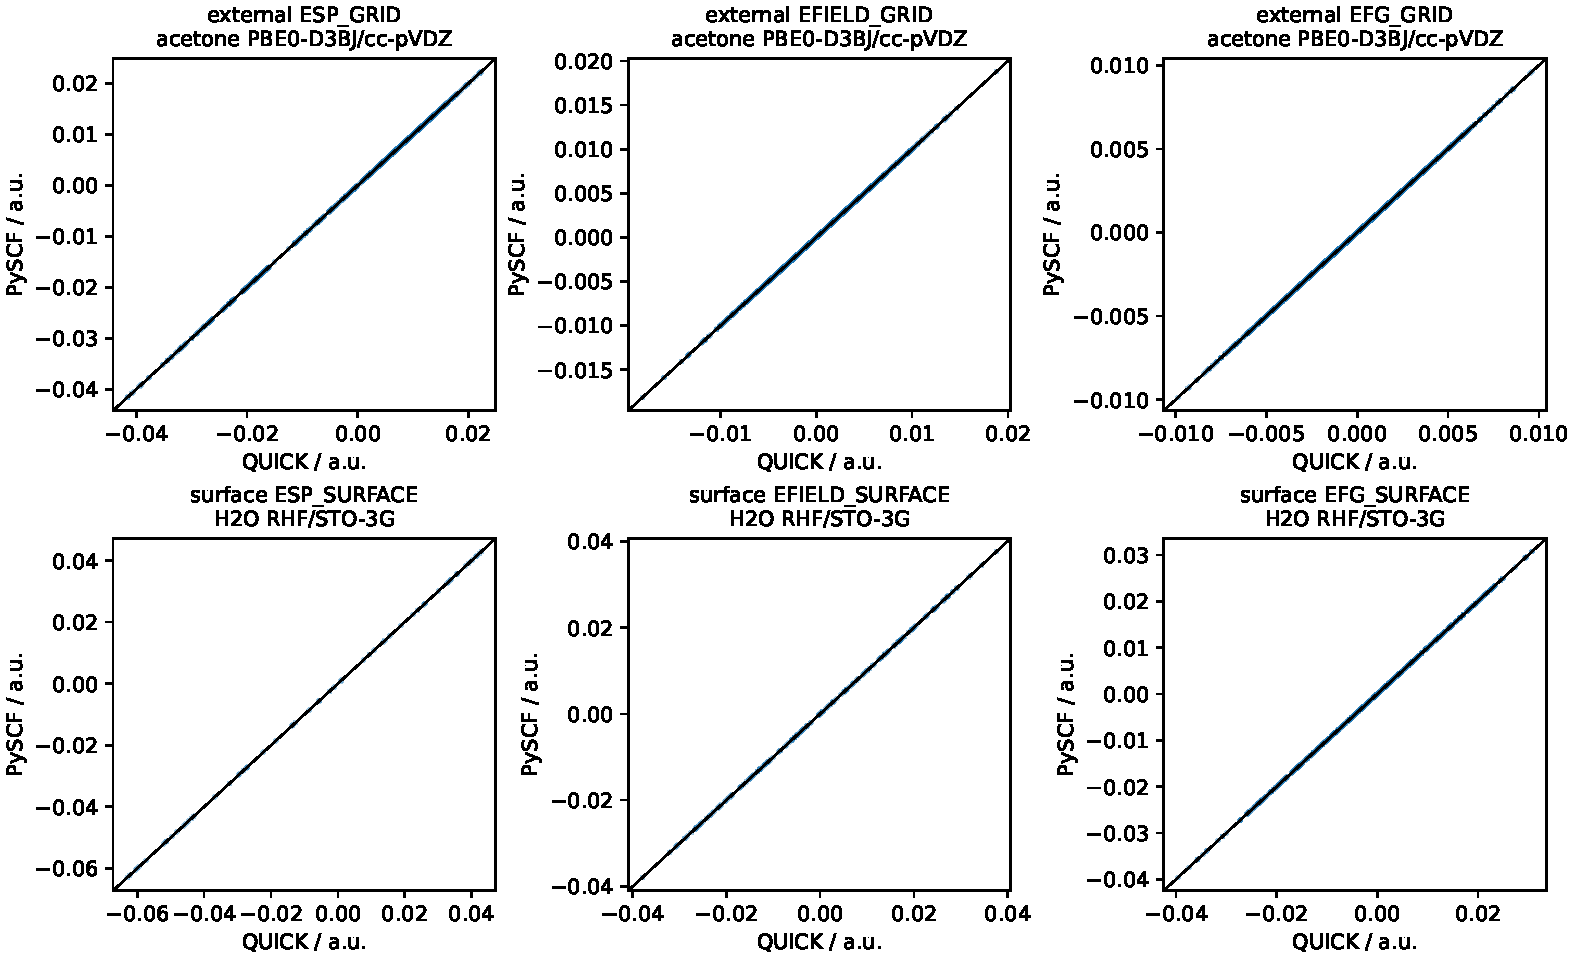
\includegraphics[width=\linewidth]{figures/pyscf_validation_scatter.pdf}
  \caption{Pointwise comparison of QUICK and PySCF electrostatic properties on the acetone PBE0-D3BJ/cc-pVDZ external grid and the water RHF/STO-3G electron-density surface.  PySCF EFIELD and EFG values are finite differences of PySCF ESP values using the QUICK sign convention.}
  \label{fig:pyscf_validation}
\end{figure}

Additional implementation details and algorithm pseudocode are provided in the Supporting Information.

\section{Potential Applications}

The combination of ESP, electric field, field-gradient tensor, and finite-field perturbation opens several compact application directions.  First, grid-based field descriptors can distinguish electrostatic environments that have similar scalar potentials but different field directionality or curvature.  Second, field-gradient eigenvalues and invariants can identify anisotropic electrostatic regions near lone pairs, pi systems, sigma holes, and polar bonds.  Third, finite-field calculations make it possible to examine induced changes in \(V(\mathbf{C})\), \(\mathbf{E}(\mathbf{C})\), and \(G_{ij}(\mathbf{C})\) from field-polarized densities.  These response descriptors can be used to identify where a molecule's local electrostatic environment is most polarizable or most field-sensitive.  Fourth, the post-SCF OEPROP evaluators and the public \texttt{getQuickOEPROP} API can be used to analyze saved molecular-dynamics trajectories frame by frame, including local electrostatics along interfacial or reactive coordinates.  The same API can be called by an external dynamics driver after each SCF or gradient step, although QUICK still lacks a complete native BOMD engine that emits OEPROP automatically at every step.  Finally, these quantities may be used as target data for next-generation charge, multipole, and polarizable models that fit not only the scalar potential but also local field and field-gradient response.

\section{Outlook}

This implementation establishes CPU serial and MPI support for scalar, vector, and tensor electrostatic grid and electron-density-surface properties in QUICK, plus finite uniform external electric fields for SCF energies and post-SCF property analysis.  Immediate next steps include CUDA/HIP-host validation of the new GPU OEPROP EFIELD/EFG kernels, replacing the reference recursive device EFG evaluator with generated derivative recurrence tables, using the public OEPROP API in external BOMD/AIMD drivers, adding compact tensor invariants to standard output, improving the density-surface sampler, extending validation across basis sets and charged/open-shell systems, and implementing analytic gradients under finite external fields.

\section{Conclusions}

QUICK now evaluates ESP, electric fields, finite-difference electric field gradients, and analytic electric field gradients on external molecular grids and internally generated electron-density isosurfaces, can apply finite uniform external electric fields during CPU serial and MPI SCF calculations, and exposes a no-I/O OEPROP API for trajectory analysis.  The analytic EFG follows an Obara-Saika recurrence for second derivatives of one-electron attraction integrals and is parallelized with the existing MPI shell-pair distribution.  The finite-field implementation uses the corresponding first-moment one-electron operator and the matching classical charge-field energy.  Agreement between analytic and numerical EFGs to printed precision, PySCF cross-code validation, serial/MPI surface-property agreement, serial/MPI finite-field agreement, file-vs-API OEPROP parity, and the expected dipole derivative check provides a stringent implementation baseline for practical grid-based, surface-based, and trajectory-based electrostatic analysis.

\begin{acknowledgement}
TODO: Add funding, software, and contributor acknowledgements.
\end{acknowledgement}

\begin{thebibliography}{9}

\bibitem{previous_jcim}
TODO: Add full citation for the preceding JCIM paper, DOI: 10.1021/acs.jcim.5c03200.

\bibitem{obara_saika}
S. Obara and A. Saika, Efficient recursive computation of molecular integrals over Cartesian Gaussian functions, \emph{J. Chem. Phys.} \textbf{1986}, \emph{84}, 3963--3974.

\bibitem{hgp}
M. Head-Gordon and J. A. Pople, A method for two-electron Gaussian integral and integral derivative evaluation using recurrence relations, \emph{J. Chem. Phys.} \textbf{1988}, \emph{89}, 5777--5786.

\bibitem{helgaker_book}
T. Helgaker, P. Jorgensen, and J. Olsen, \emph{Molecular Electronic-Structure Theory}; Wiley: Chichester, 2000.

\bibitem{quick}
TODO: Add current QUICK citation and version citation.

\end{thebibliography}

\end{document}
